	Supervised Learning gehört zu den erfolgreichsten und meist verbreiteten Arten des Machine Learnings. \cite{Mueller2016}
	Beim Supervised Learning werden bekannte Daten und Ausgaben während dem Trainieren und Prüfen des Modells genutzt, welche auch Trainings-Daten und Label genannt werden. \cite{Sarkar2018} Diese optimieren das Modell, auf Basis der vorhandenen Daten, durch Anpassen der Parameter. \cite{Suthaharan2016} Ein Modell besteht aus den in- und output-Paaren des Training Datensatzes. \cite{Mueller2016} Das Hauptziel ist es die eingehenden Daten x auf die ausgehenden y abzubilden (f(x) = y), um später für neue Daten x' die zugehörigen Daten y' zu bestimmen.\cite{Sarkar2018}
	Durch eine größere Menge an Trainings-Daten ist eine bessere Abdeckung von verschiedenen Fällen möglich, dies kann aber auch zu Overfitting führen. Um das zu verhindern muss das Training früh genug beendet werden. \cite{Suthaharan2016} Bei Overfitting werden die Daten sozusagen auswendig gelernt. Sollen neue Daten analysiert werden kommt es hierbei oft zu Fehlern. \cite{Kirk2014} Overfitting entsteht durch zu viele Parameter. Der Gegensatz zu Overfitting ist Underfitting. Hier ist das Modell zu einfach, es hat also zu wenige oder schlechte Parameter. \cite{Geron2017} Das Modell kann somit keine akkurate Nachbildung liefern. Sind von einer Exponentialfunktion nur zwei Punkte gegeben, könnte die Funktion als Gerade interpretiert werden. Alle anderen Punkte, die das Modell liefert, sind dadurch nicht korrekt. \cite{Kirk2014}
	Es gibt zwei Methoden für Supervised Learning: Klassifikation und Regression. Die Wahl der Methode hängt von der zu erfüllenden Aufgabe ab.\cite{Sarkar2018}
	
	\subsection{Klassifikation}
	
	Das Ziel der Klassifikation ist es ein Klassenlabel für die eingehenden Daten vorauszusagen. Die verschiedenen Label sind Teil einer vorgegebenen Liste. \cite{Mueller2016} Die Klassifikation kann in binäre und multiklassen Klassifkation aufgeteilt werden. Bei binärer Klassifikation sind nur zwei Klassen verfügbar, die Problemstellung lässt sich also auf eine Ja/Nein-Frage ableiten, die aussagt ob der Datensatz zu einer Klasse A gehört oder nicht und somit in Klasse B eingeordnet werden muss. Ein Beispiel hierfür ist das Verarbeiten von Daten einer Wettervorhersage(siehe \ref{fig:abb1}). Aus den eingehenden Daten(Temperatur und Luftfeuchtigkeit) entscheidet das Supervised Modell ob es sich um die Klasse Sonne oder Regen handelt.  \cite{Mueller2016}\newline 
		\begin{figure}[H]
			\centering
			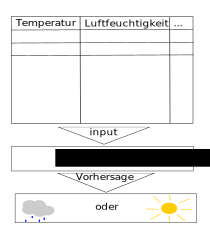
\includegraphics[width=6cm]{Bilder/Label.pdf}
			\caption{Beispiel Wettervorhersage}
			\label{fig:abb1}
		\end{figure}
		
	In der multiklassen Klassifikation können die Inputdaten auf mehr als zwei Klassen aufgeteilt werden, es handelt sich also nicht mehr um eine Ja/Nein-Frage. \cite{Mueller2016} Während der Trainings-Phase werden Regeln für das Zuteilen von Labels erstellt, die später dabei helfen Test-Daten Labels zuzuweisen.  \cite{Suthaharan2016}
	
	\subsubsection{Support Vector Machines}
	Support Vector Maschinen oder auch kurz SVMs, sind vielseitige und mächtige Machine Learning Modelle. Sie zählen zu den beliebtesten Modellen und eignen sich für lineare und nicht-lineare Klassifikation, Regression und zum Erkennen von Anomalien. \cite{Geron2017} SVMs können mathematisch sehr komplex sein und eine hohe Rechenleistung erfordern. \cite{Suthaharan2016} Im Folgenden wird nur die lineare Klassifikation betrachtet.\newline
	Hier ist es möglich zwei Klassen durch eine lineare Trennline eindeutig zu trennen. Diese soll einen Möglichst großen Abstand zu den Datensätzen haben, um später beim Einfügen neuer Daten weniger Fehler zu erzielen.\cite{Geron2017} Da die Trennlinie linear ist, lässt sie sich durch den Term 
		\begin{equation}
		0 = wx^{'} + \gamma
		\end{equation}
	beschreiben. \cite{Suthaharan2016} Der Abstand der Trennlinie zu den beiden nächsten Punkten, die aus verschiedenen Klassen stammen, nennt sich Margin. Die Geraden parallel zur Trennline, durch die zwei Punkte, die diese Grenze bilden, heißen Support Vektoren. In Abbildung \ref{fig:abb10} ist die Trennline die durchgezogene Linie und die Support Vektoren die gestrichelten Linien, der Margin befindet sich zwischen ihnen. Werden während dem Training neue Daten hinzugefügt, die sich außerhalb des Margins befinden, wird das Modell nicht geändert. \cite{Geron2017} Beim Training werden w und $\gamma$ optimiert. \cite{Suthaharan2016}\newline
	
	\begin{figure}[H]
		\centering
		\includegraphics[width=5cm]{Bilder/SVM.pdf}
		\caption{SVM Trennline und Datensätze}
		\label{fig:abb10}
	\end{figure}
	
	Im Folgenden wird mit der scikit-learn Bibliothek ein SVM-Modell erstellt und mit der Funktion fit trainiert. X\_train und y\_train beinhalten die Trainings-Datensätze. Mit Hilfe von predict kann ein neuer Datensatz klassifiziert werden.
	\lstset{style=code}
	\begin{lstlisting}[language=Python]
	def_svc = SVC()
	def_svc.fit(X_train, y_train)
	def_y_pred = def_svc.predict(X_test)
	\end{lstlisting}
	\cite{Sarkar2018}	
	 
	
	\subsection{Regression}
	In Regressions-Problemen sollen oft Zahlen oder Werte ermittelt werden. Im Gegensatz zur Klassifikation gibt es keine Klassen oder Label, denen Daten zugeordnet werden können. Regressions-Modelle lernen stattdessen den Zusammenhang aus Ein- und Ausgangsdaten, um für neue Daten den passenden Output vorherzusagen. \cite{Sarkar2018}
	 \newline
	Abbildung \ref{fig:abb2} zeigt ein Beispiel bei dem mit Hilfe von Datensätzen, die Informationen zu Eiskäufen pro Minute und der Temperatur enthalten, eine Funktion gelernt werden konnte, um für zukünftige Temperaturen die passende Anzahl an Eiskäufen pro Minute auszugeben. \cite{Sarkar2018}
	\newline
	
	\begin{figure}[H]
		\centering
		\includegraphics[width=5cm]{Bilder/Regression.pdf}
		\caption{Beispiel Regression}
		\label{fig:abb2}
	\end{figure}
	
	Lineare Regressions Modelle versuchen mit nur einer Variable x eine Output-Variable y zu bestimmen und können somit lineare Probleme lösen. \cite{Sarkar2018}
	\newline
	Multivariable Regressions Methoden werden für Probleme mit mehreren input-Variablen in Form eines Vektors und nur einer output-Variable verwendet. \cite{Sarkar2018}
	 \newline
	Ein Sonderfall der Multivariablen Regression ist die Polynomiale Regression. Hier ist die Ausgabevariable Polynom n-ten Grades der Eingangsvariable. \cite{Sarkar2018}
	\newline
	Nichtlineare Regressions Modelle stellen zwischen ein- und ausgehenden Daten eine Beziehung auf Basis einer Kombination aus nicht-linearen Funktionen her. \cite{Sarkar2018}
	\newline
	%Lasso regression is a special form of regression that performs normal regression and generalizes the
	%model well by performing regularization as well as feature or variable selection. Lasso stands for least absolute
	%shrinkage and selection operator. The L1 norm is typically used as the regularization term in lasso regression
	%Ridge regression is another special form of regression that performs normal regression and generalizes
	%the model by performing regularization to prevent overfitting the model. Typically the L2 norm is used as the
	%regularization term in ridge regression 
	%Generalized linear models are generic frameworks that can be used to model data predicting different
	%types of output responses, including continuous, discrete, and ordinal data. Algorithms like logistic
	%regression are used for categorical data and ordered probit regression for ordinal data.(Sarkar, S.38)
	
	